\begin{frame}
\frametitle{\charm}
\framesubtitle{}
	\begin{block}{What is it?}
	\begin{columns}
	\begin{column}{0.5\textwidth}
		\begin{itemize}
		\item Programming model
		\item Programming framework
		\item Runtime system software
	\end{itemize}
	\end{column}
	\begin{column}{0.3\textwidth}
		{\Large designed for parallelism}
	\end{column}
	\end{columns}
	\end{block}
    \begin{itemize}
        \item General-purpose C++ parallel programming framework
        \item Abstracts parallel algorithm design from concrete hardware
        \item Shared-nothing by default, explicit sharing for optimization
        \item Abstracts domain logic from parallel tuning
        \item Rich ecosystem of runtime and tool support to address domain-independent
          concerns
    \end{itemize}
\end{frame}


\begin{frame}
\frametitle{\charm: Some Capabilities}
\framesubtitle{Transparent to application code!}
    \begin{itemize}
        \item Seamless parallel composability of modular components
        \item Fault tolerance
        \item Dynamic load balancing
        \item Energy management
    \end{itemize}
\end{frame}


\begin{frame}
\frametitle{\charm: Portability}
\only<1>{
\framesubtitle{Environments}
    \begin{itemize}
        \item Embedded ARM: cell phones, CARMA dev boards
        \item Commodity x86: servers, desktops, laptops, tablets
        \item Clusters: commodity, with a network
        \item Supercomputers: IBM Blue Gene and POWER, Cray
    \end{itemize}
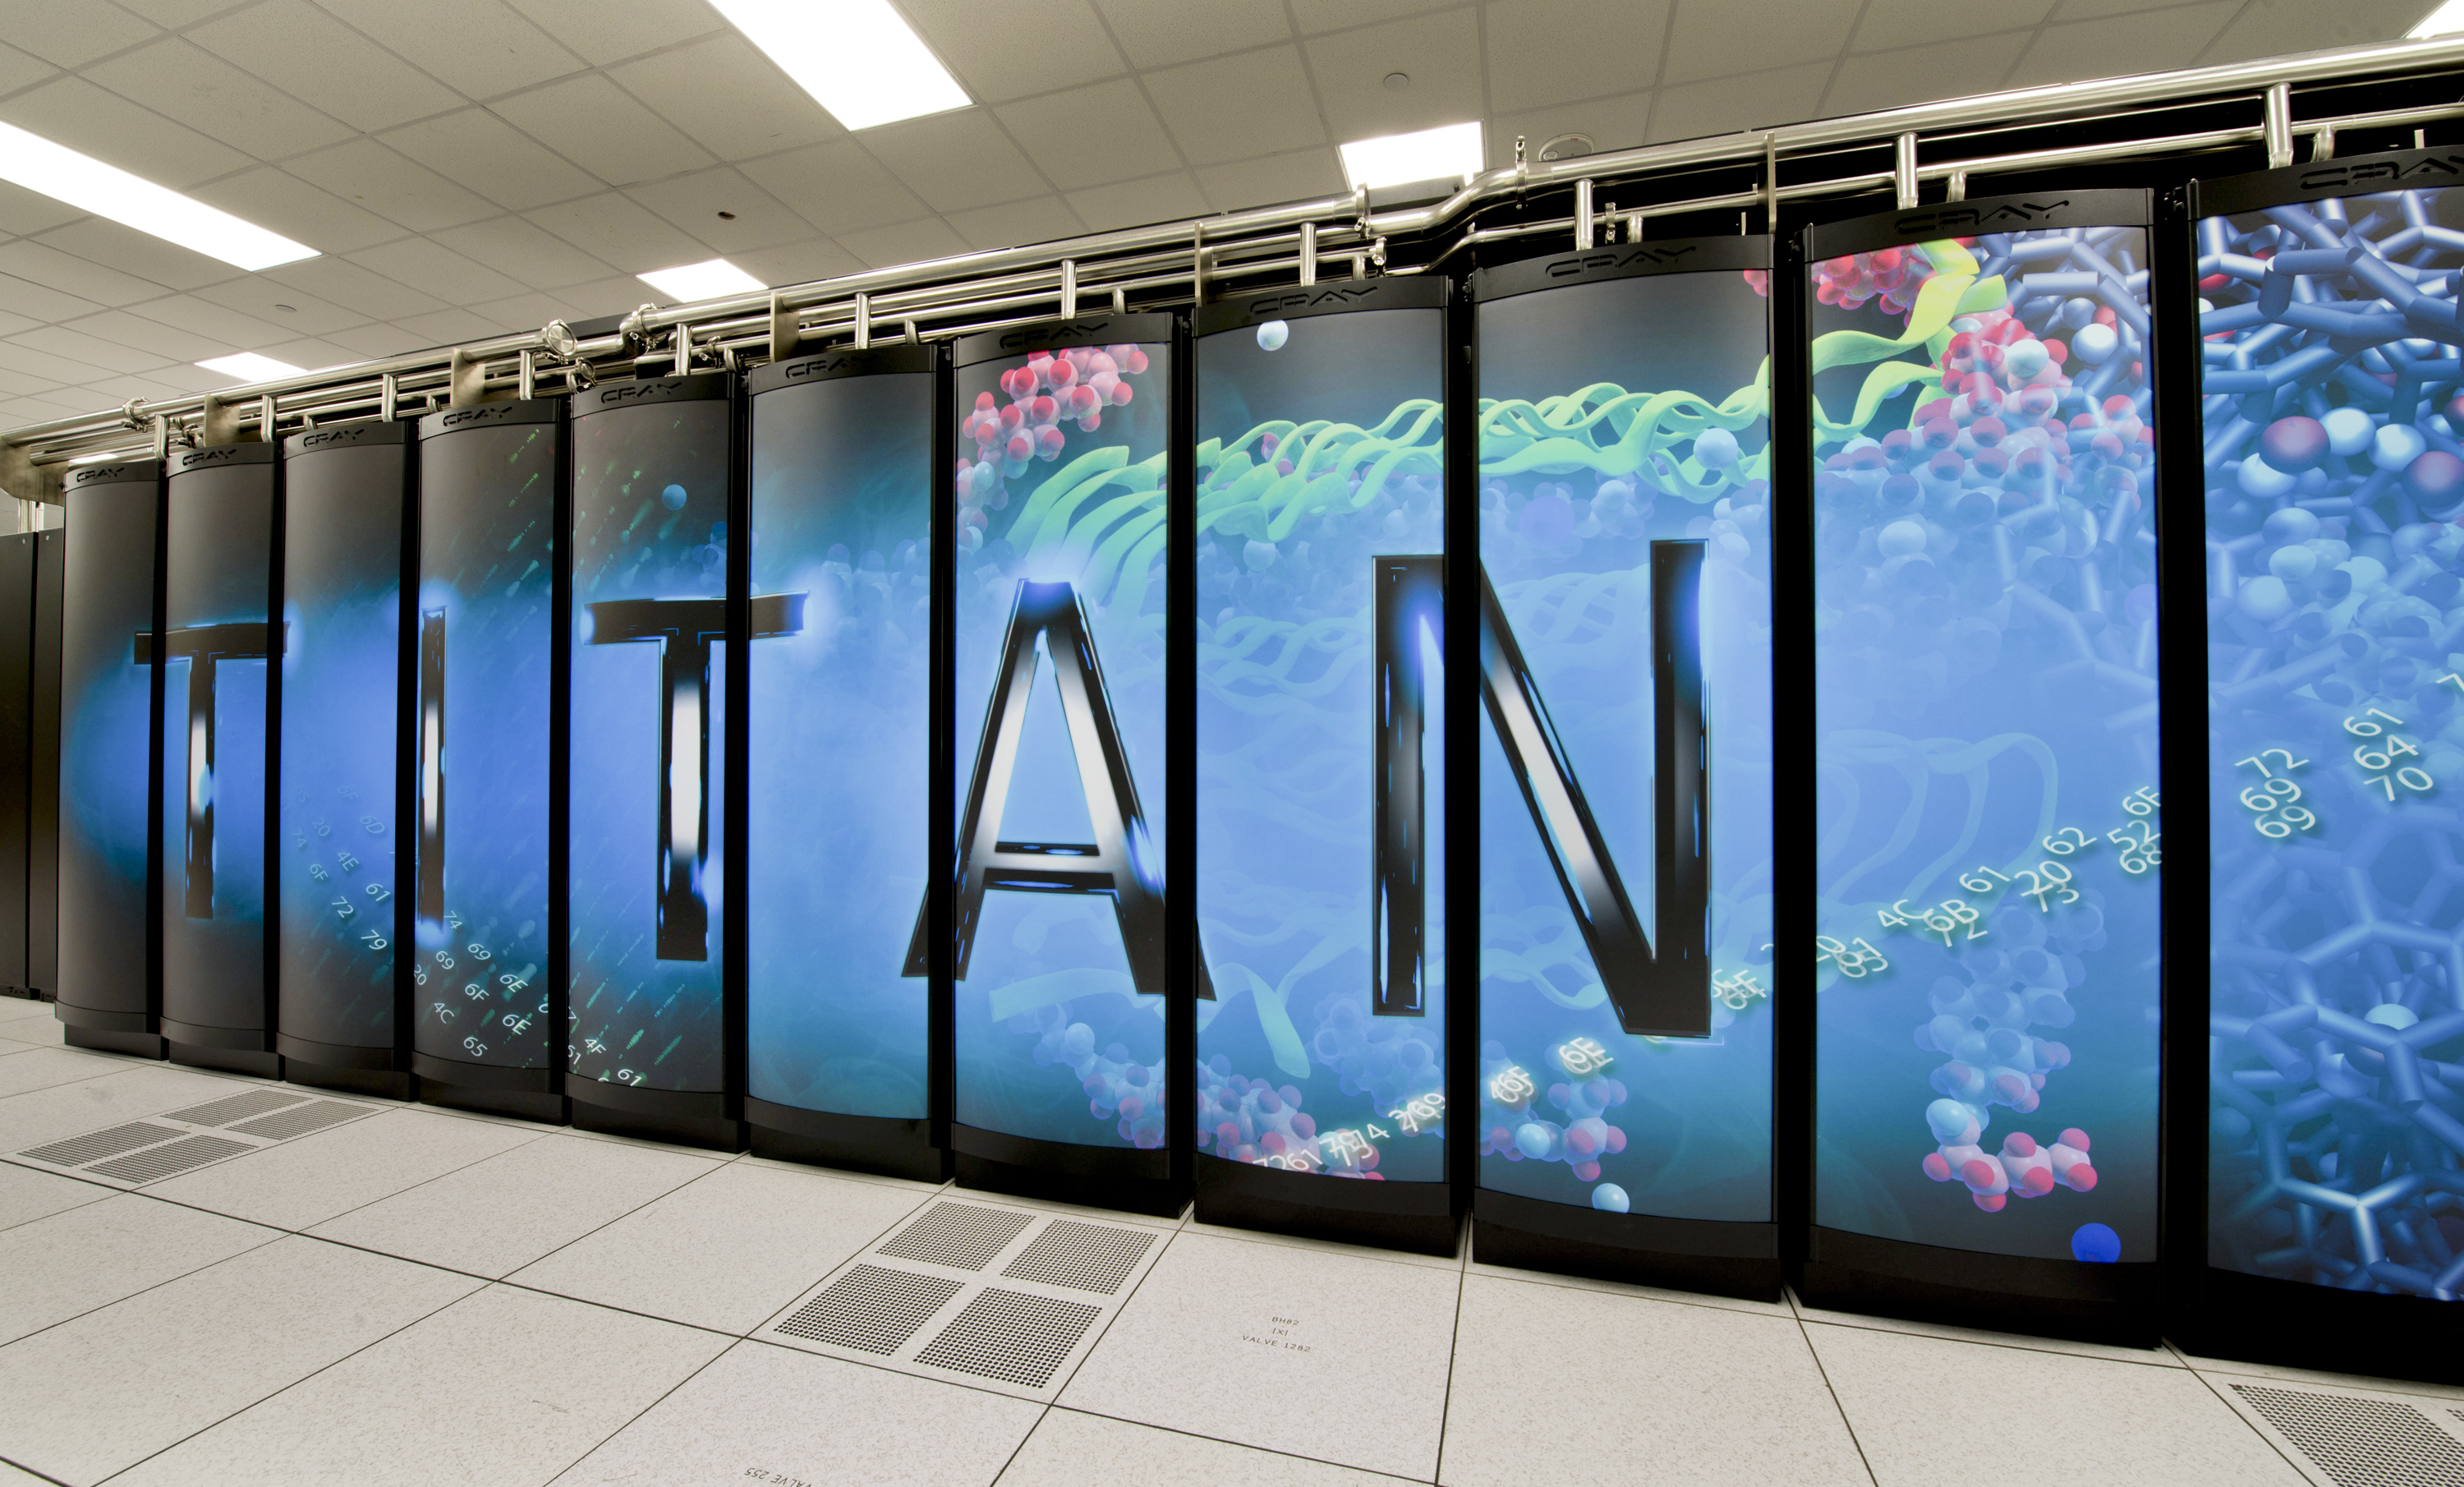
\includegraphics[scale=0.07]{../figures/titan.jpg}
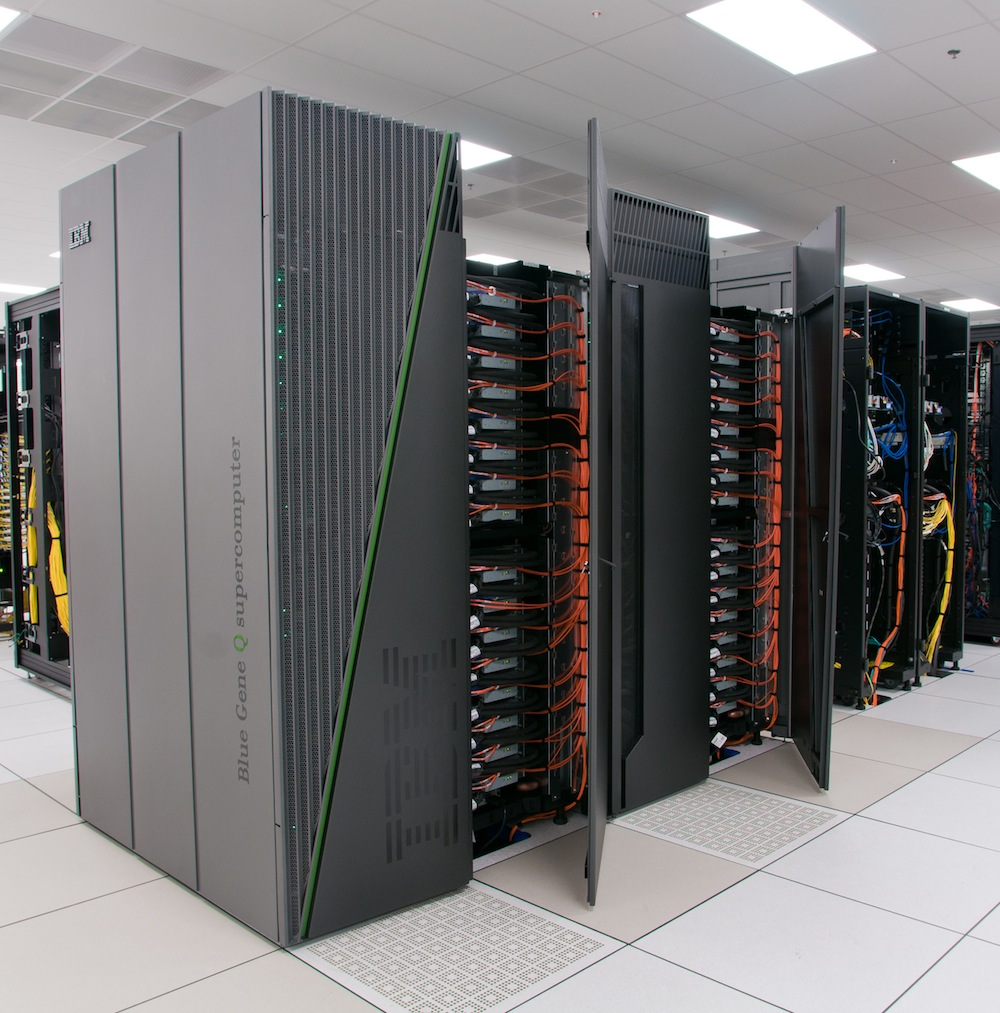
\includegraphics[scale=0.5]{../figures/mira.jpg}
}
\only<2>{
  \framesubtitle{Operating Systems}
  \begin{itemize}
  \item Linux
  \item Mac OS X
  \item Windows
  \item Proprietary Cray \& IBM
  \end{itemize}
}
\only<3>{
  \framesubtitle{Network Interfaces}
  \begin{itemize}
    \item TCP, UDP
    \item Shared memory
    \item MPI
    \item Infiniband Verbs
    \item Native Blue Gene P (DCMF), Blue Gene Q (PAMI)
    \item Native Cray Gemini and Aries (uGNI)
  \end{itemize}
}
\only<4>{
\framesubtitle{Compilers}
\begin{itemize}
\item GCC
\item Clang
\item Microsoft VC++
\item IBM XL
\item Intel
\item Portland Group (PGI)
\item Cray
\item Fujitsu
\end{itemize}
}
\end{frame}

\begin{frame}
\frametitle{\charm: Pedigree}
\begin{itemize}
\item Precursors: Rediflow (Keller), Actors, ABCL (Yonezawa)
\item 1987: Chare Kernel arose from parallel Prolog work
\item 1992: Initial C++-based Charm++
\item 1994-1996: NAMD developed
\item 1997: Application-facing abstractions reach near-current form
\item 1997: Adaptive MPI (AMPI) built atop Charm++
\item 2000-present: More applications developed, runtime facilities extended,
  sacling with new machines
\end{itemize}
\end{frame}
